% Especificaciones del tamaño de letra, tamaño de hoja, márgenes, librerias, etc.
\documentclass[12pt, letterpaper]{article}
\usepackage[english]{babel}
\usepackage{fancyhdr}
\usepackage[utf8]{inputenc}
\usepackage[T1]{fontenc}
\usepackage{amsmath}
\usepackage{graphicx}
\usepackage{subcaption}
\usepackage[hidelinks]{hyperref}
\usepackage{url}
\usepackage{amssymb}
\usepackage{float}
\usepackage[margin=1in]{geometry}
\renewcommand{\baselinestretch}{1.5}

% Enlace Bibliografía
\usepackage{csquotes}
\usepackage[backend=biber]{biblatex}
\addbibresource{referencias.bib}

% Titulo, autores, fecha.
\title{Homework \#2: Mohr's Circle}
\author{Carlos A. Vásquez Castañeda \and 1155057 \and Group 393}
\date{October 14, 2019}
\pagestyle{fancy}
\fancyhf{}
\rhead{Aircraft Elements Design}
\lhead{Mohr's Circle}
\rfoot{\thepage}


% Inicio del documento
\begin{document}
\maketitle
Calculating stresses tends to be straight fordward whenever the loads being applied are in the same line of action because with the superposition of these stresses one can easily find the maximum normal stress (e.g., a beam in which there's a stress acting normal to one axis and a bending stress). However, when a torque is applied we can't continue to apply this superposition method in order to find the maximum normal or shear stresses, as seen in figure 1.

\begin{figure}[H]
	\centering
	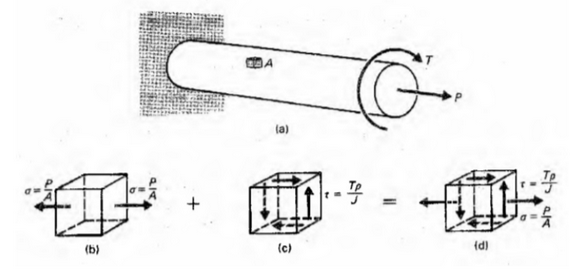
\includegraphics[width=\textwidth]{stress.png}
	\caption{It's not possible to add both stresses.}
\end{figure}

The principal plane is the plane of the stress element (labeled as A in the figure) in which there are no shear stresses being applied to it, only normal stresses. That is, the plane that holds the maximum normal stress. This stress element will be at an angle, and the maximum shear stress will be at an angle of 45º with respect to the angle of the principal planes. This facts are really useful when analyizing different kinds of materials. 

When having a ductile material, they fail with neck formation of the material, and these necks form thanks to the action of the shear stresses present in the material, specifically thanks to the action of the maximum shear stresses. Similarly, brittle materials fail due to maximum normal stresses, which, when applying different loads to the material, will appear usually at an angle.

The method utilised to find these maximum shear and normal stresses is usually analyzing sections of the stress element making an angle via the stress transformation equations:

\begin{equation}
	\begin{split}
		\sigma &= \frac{\sigma_x + \sigma_y}{2} + \frac{\sigma_x - \sigma_y}{2}\cos 2\theta + \tau_{xy}\sin 2\theta\\
		\tau &= -\frac{\sigma_x - \sigma_y}{2}\sin 2\theta + \tau_{xy}\cos 2\theta
	\end{split}
\end{equation}
And in order to find the maximum sheer and normal stresses, along with the angle at which these happen, we use the following formulas:

\begin{equation}
	\begin{split}
		\tau_{max} &= \sqrt{(\frac{\sigma_x - \sigma_y}{2})^2 + \tau_{xy}^2}\\
		\sigma_{1,2} &= \frac{\sigma_x + \sigma_y}{2} \pm \sqrt{(\frac{\sigma_x - \sigma_y}{2})^2 + \tau_{xy}^2}\\
		\tan 2\theta_p &= \frac{\tau_{xy}}{(\sigma_x - \sigma_y)/2}
	\end{split}
\end{equation}

These formulas are easily calculated by a computer or a calculator, however they are still pretty convoluted (and the formulas above are just for the 2-dimensional normal and shear stress). An easier way of calculating the maximum normal and shear stresses are through what's known as Mohr's Circle.

Mohr's circle consists in the parametric representation of a circle where the axes are the normal stress and shear stress ($\sigma$ and $\tau$), and their values are completely dependent on the angle $\theta$, as shown in the figure below.

\begin{figure}[H]
	\centering
	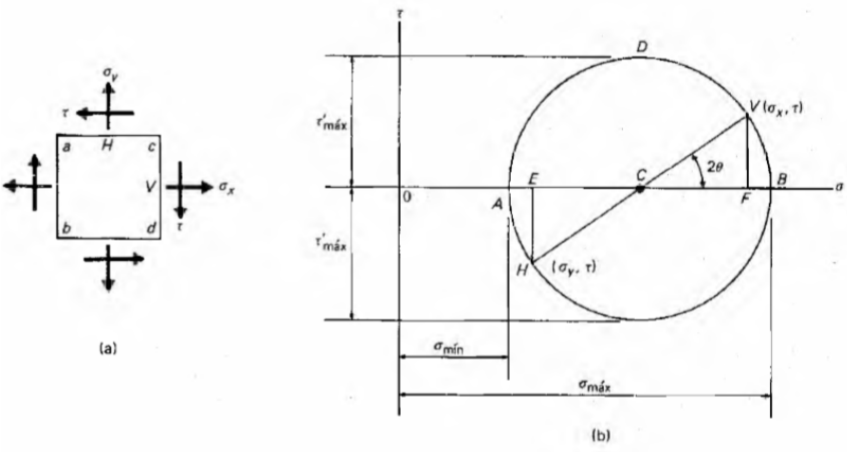
\includegraphics[width=\textwidth]{circ.png}
	\caption{Construction of a Mohr's circle for the 2-dimensional stress element.}
\end{figure}

We will illustrate through an example the usage of Mohr's circle. We will determine the principal normal stresses, the principal shear stress and the angle at which these happen in the stress element given below via Mohr's circle.
\begin{figure}[H]
	\centering
	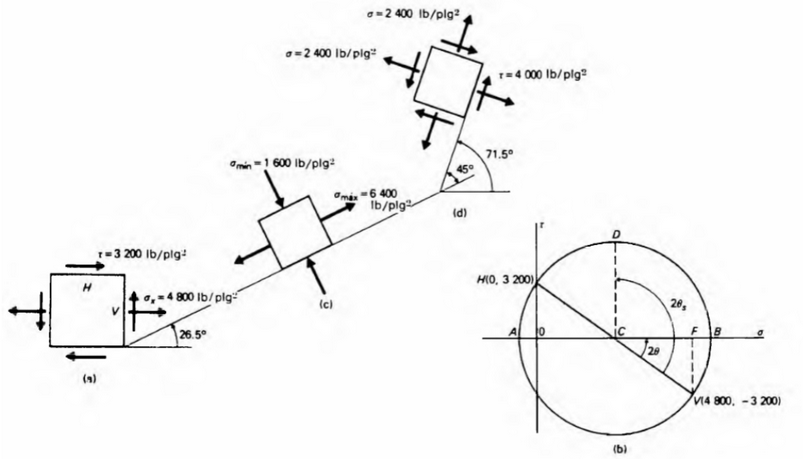
\includegraphics[width=0.9\textwidth]{ex.png}
	\caption{Stress element and its corresponding Mohr's circle.}
\end{figure}

As figure 2 suggests, the points V and H are already known thanks to figure 3(a), as it shows the normal and shear stresses. The midpoint between these points will the the center which we'll call point C (or distance OC). Thus the point C will be located at C(2400, 0). In order to obtain the maximum principal normal stress, it is possible to calculate the distance OB:
\begin{equation}
	\begin{split}
		OB &= OC +\ radius\\
		&= OC + \sqrt{CF^2 + FV^2}\\
		&= 2400 + \sqrt{2400^2 + (-3200)^2}\\
		&= 2400 + 4000\\
		\sigma_1 &= 6400\ psi
	\end{split}
\end{equation}

Likewise, to obtain the minimum principal normal stress we need to calculate the distance OA like so:

\begin{equation}
	\begin{split}
		OA &= OC -\ radius\\
		&= OC - \sqrt{CF^2 + FV^2}\\
		&= 2400 - \sqrt{2400^2 + (-3200)^2}\\
		&= 2400 - 4000\\
		\sigma_2 &= -1600\ psi
	\end{split}
\end{equation}

Now, in order to obtain the angle made with respect to the reference angle, we need to look at the circle and remember that every rotation made in it will be 2 times the one we actually need to make. Therefore, by trigonometry:

\begin{equation}
	\tan(2\theta) = \frac{FV}{CF} = \frac{3200}{2400} = 1.33
\end{equation}

Solving for the angle we'll have

\begin{equation}
	\begin{split}
		2\theta &= \arctan 1.33 = 53º\\
		\theta &= 26.5º
	\end{split}
\end{equation}

Lastly, given that point D is where maximum shear stress occurs, we observe that $2\theta_S = 2\theta + 90º$. And taking into account that point D is in D(2400, 4000), we can conclude that:

\begin{equation}
	\theta_S = \theta + 45º = 71.5º
\end{equation}

To better illustrate these results, consider the figure shown below. Here we see the inclination angles and the maximum stresses. In (a) we can see the maximum and minimum principal normal stresses due to the inclination angle, and in (b) we see the maximum shear stress. Mohr's circle is possible thanks to the nature of the equations utilised to calculate the principal stresses.\supercite{fitz82}

\begin{figure}
	\centering
	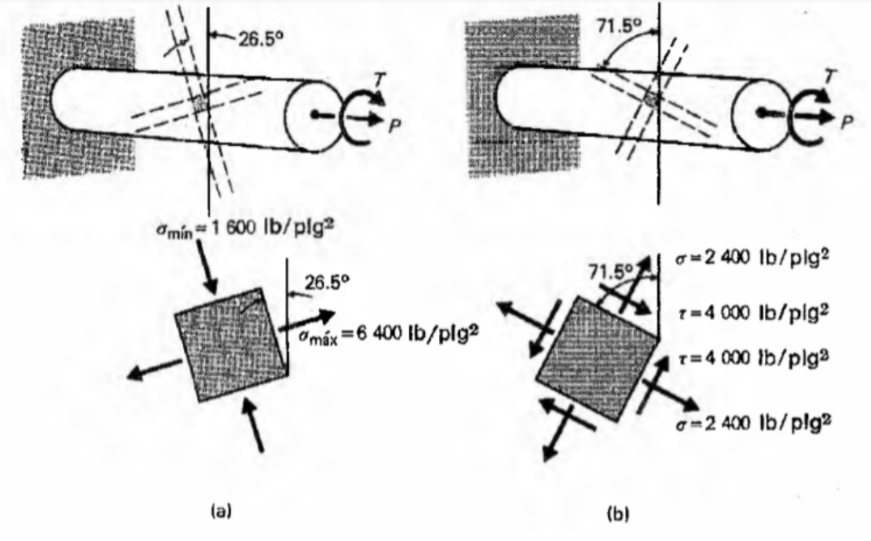
\includegraphics[width=\textwidth]{ang.png}
	\caption{Corresponding stresses and angles.}
\end{figure}
%%%%%  Bib
\renewcommand\refname{References}
\printbibliography
\end{document}
